%!TeX encoding = UTF-8
%!TeX program = xelatex
\documentclass[notheorems, aspectratio=54]{beamer}
% aspectratio: 1610, 149, 54, 43(default), 32
\usepackage{pgfplots}

\usepackage{latexsym}
\usepackage{amsmath,amssymb}
\usepackage{mathtools}
\usepackage{color,xcolor}
\usepackage{graphicx}
\usepackage{algorithm}
\usepackage{amsthm}
\usepackage{lmodern} % 解决 font warning
% \usepackage[UTF8]{ctex}
\usepackage{animate} % insert gif

\usepackage{lipsum} % To generate test text 
\usepackage{ulem} % 下划线,波浪线

\usepackage{listings} % display code on slides; don't forget [fragile] option after \begin{frame}

\usepackage{tkz-euclide}

% arrow and line for 'tkzPointShowCoord'
\makeatletter
\tikzset{arrow coord style/.style={%
    densely dashed,
    \tkz@euc@linecolor,
    %>=stealth',
    %->,
    }}
    \tikzset{xcoord style/.style={%
    \tkz@euc@labelcolor,
    font=\normalsize,text height=1ex,
    inner sep = 0pt,
    outer sep = 0pt,
    fill=\tkz@fillcolor,
    below=6pt
    }} 
\tikzset{ycoord style/.style={%
    \tkz@euc@labelcolor,
    font=\normalsize,text height=1ex, 
    inner sep = 0pt,
    outer sep = 0pt, 
    fill=\tkz@fillcolor,
    left=6pt
    }}  
\makeatother
% ----------------------------------------------
% tikx
\usepackage{framed}
\usepackage{tikz}
\usepackage{pgf}
\usetikzlibrary{automata, calc,trees,positioning,arrows,chains,shapes.geometric,%
    decorations.pathreplacing,decorations.pathmorphing,shapes,%
    matrix,shapes.symbols}
\pgfmathsetseed{1} % To have predictable results
% Define a background layer, in which the parchment shape is drawn
\pgfdeclarelayer{background}
\pgfsetlayers{background,main}

% define styles for the normal border and the torn border
\tikzset{
  normal border/.style={orange!30!black!10, decorate, 
     decoration={random steps, segment length=2.5cm, amplitude=.7mm}},
  torn border/.style={orange!30!black!5, decorate, 
     decoration={random steps, segment length=.5cm, amplitude=1.7mm}}}

% Macro to draw the shape behind the text, when it fits completly in the
% page
\def\parchmentframe#1{
\tikz{
  \node[inner sep=2em] (A) {#1};  % Draw the text of the node
  \begin{pgfonlayer}{background}  % Draw the shape behind
  \fill[normal border] 
        (A.south east) -- (A.south west) -- 
        (A.north west) -- (A.north east) -- cycle;
  \end{pgfonlayer}}}

% Macro to draw the shape, when the text will continue in next page
\def\parchmentframetop#1{
\tikz{
  \node[inner sep=2em] (A) {#1};    % Draw the text of the node
  \begin{pgfonlayer}{background}    
  \fill[normal border]              % Draw the ``complete shape'' behind
        (A.south east) -- (A.south west) -- 
        (A.north west) -- (A.north east) -- cycle;
  \fill[torn border]                % Add the torn lower border
        ($(A.south east)-(0,.2)$) -- ($(A.south west)-(0,.2)$) -- 
        ($(A.south west)+(0,.2)$) -- ($(A.south east)+(0,.2)$) -- cycle;
  \end{pgfonlayer}}}

% Macro to draw the shape, when the text continues from previous page
\def\parchmentframebottom#1{
\tikz{
  \node[inner sep=2em] (A) {#1};   % Draw the text of the node
  \begin{pgfonlayer}{background}   
  \fill[normal border]             % Draw the ``complete shape'' behind
        (A.south east) -- (A.south west) -- 
        (A.north west) -- (A.north east) -- cycle;
  \fill[torn border]               % Add the torn upper border
        ($(A.north east)-(0,.2)$) -- ($(A.north west)-(0,.2)$) -- 
        ($(A.north west)+(0,.2)$) -- ($(A.north east)+(0,.2)$) -- cycle;
  \end{pgfonlayer}}}

% Macro to draw the shape, when both the text continues from previous page
% and it will continue in next page
\def\parchmentframemiddle#1{
\tikz{
  \node[inner sep=2em] (A) {#1};   % Draw the text of the node
  \begin{pgfonlayer}{background}   
  \fill[normal border]             % Draw the ``complete shape'' behind
        (A.south east) -- (A.south west) -- 
        (A.north west) -- (A.north east) -- cycle;
  \fill[torn border]               % Add the torn lower border
        ($(A.south east)-(0,.2)$) -- ($(A.south west)-(0,.2)$) -- 
        ($(A.south west)+(0,.2)$) -- ($(A.south east)+(0,.2)$) -- cycle;
  \fill[torn border]               % Add the torn upper border
        ($(A.north east)-(0,.2)$) -- ($(A.north west)-(0,.2)$) -- 
        ($(A.north west)+(0,.2)$) -- ($(A.north east)+(0,.2)$) -- cycle;
  \end{pgfonlayer}}}
% Define the environment which puts the frame
% In this case, the environment also accepts an argument with an optional
% title (which defaults to ``Example'', which is typeset in a box overlaid
% on the top border
\newenvironment{parchment}[1][Example]{%
  \def\FrameCommand{\parchmentframe}%
  \def\FirstFrameCommand{\parchmentframetop}%
  \def\LastFrameCommand{\parchmentframebottom}%
  \def\MidFrameCommand{\parchmentframemiddle}%
  \vskip\baselineskip
  \MakeFramed {\FrameRestore}
  \noindent\tikz\node[inner sep=1ex, draw=black!20,fill=white, 
          anchor=west, overlay] at (0em, 2em) {\sffamily#1};\par}%
{\endMakeFramed}

% ----------------------------------------------

\mode<presentation>{
    \usetheme{CambridgeUS}
    % Boadilla CambridgeUS
    % default Antibes Berlin Copenhagen
    % Madrid Montpelier Ilmenau Malmoe
    % Berkeley Singapore Warsaw
    \usecolortheme{beaver}
    % beetle, beaver, orchid, whale, dolphin
    \useoutertheme{infolines}
    % infolines miniframes shadow sidebar smoothbars smoothtree split tree
    \useinnertheme{circles}
    % circles, rectanges, rounded, inmargin
}
% 设置 block 颜色
\setbeamercolor{block title}{bg=red!30,fg=white}

\newcommand{\reditem}[1]{\setbeamercolor{item}{fg=red}\item #1}

% 缩放公式大小
\newcommand*{\Scale}[2][4]{\scalebox{#1}{\ensuremath{#2}}}

% 解决 font warning
\renewcommand\textbullet{\ensuremath{\bullet}}

% ---------------------------------------------------------------------
% flow chart
\tikzset{
    >=stealth',
    punktchain/.style={
        rectangle, 
        rounded corners, 
        % fill=black!10,
        draw=white, very thick,
        text width=6em,
        minimum height=2em, 
        text centered, 
        on chain
    },
    largepunktchain/.style={
        rectangle,
        rounded corners,
        draw=white, very thick,
        text width=10em,
        minimum height=2em,
        on chain
    },
    line/.style={draw, thick, <-},
    element/.style={
        tape,
        top color=white,
        bottom color=blue!50!black!60!,
        minimum width=6em,
        draw=blue!40!black!90, very thick,
        text width=6em, 
        minimum height=2em, 
        text centered, 
        on chain
    },
    every join/.style={->, thick,shorten >=1pt},
    decoration={brace},
    tuborg/.style={decorate},
    tubnode/.style={midway, right=2pt},
    font={\fontsize{10pt}{12}\selectfont},
}
% ---------------------------------------------------------------------

% code setting
\lstset{
    language=C++,
    basicstyle=\ttfamily\footnotesize,
    keywordstyle=\color{red},
    breaklines=true,
    xleftmargin=2em,
    numbers=left,
    numberstyle=\color[RGB]{222,155,81},
    frame=leftline,
    tabsize=4,
    breakatwhitespace=false,
    showspaces=false,               
    showstringspaces=false,
    showtabs=false,
    morekeywords={Str, Num, List},
}

% ---------------------------------------------------------------------

%% preamble
\title{Basic Statistics and Random Process}
% \subtitle{The subtitle}
\author{Dihui Lai}
\institute[WUSTL]{dlai@wustl.edu}

% -------------------------------------------------------------

\begin{document}

%% title frame
\begin{frame}
    \titlepage
\end{frame}

%% normal frame
\section{Introduction to Statistics: Random Variable}
\begin{frame}
CONTENT
\begin{itemize}
\item Introduction to Statistics: Random Variable
\item Empirical View of Random Variable
\item Common Probability Distributions
\item Random Walk, i.i.d and Central Limit Theorem
\end{itemize}
\end{frame}

\begin{frame}

\begin{center}
\bf{Introduction to Statistics: Random Variable}
\end{center}

\end{frame}


\begin{frame}
\begin{parchment}[Example 1: Roll a dice]
There six possible outcome of rolling a dice i.e. "1", "2", "3", ... "6".  
\begin{itemize}
\item If I roll a dice 60 times, how many times do you get "1"?
\item What is the probability of getting "1"? 1/6?
\end{itemize}
\end{parchment}
\end{frame}

\begin{frame}
\begin{parchment}[Example 2: Life time of a light bulb]
A light bulb can go broken while use. The longer it is used, the more likely the bulb will break.
\begin{itemize}
\item The value does not need to be an integer, it can be 120 hours, 120.513 hours
\item What's the probability of a light bulb breaks at the 100th hour? 1/100?

\end{itemize}
\end{parchment}
\end{frame}


\begin{frame}
\frametitle{Random Variable}

A \textbf{random variable} X can take different values with certain probability. To understand a random variable, we need to consider two things: 
\begin{itemize}
\item The possible outcome value of an experiment: $x$ 
\item The probability that an outcome is $x$.

\end{itemize}

\end{frame}


\begin{frame}
\frametitle{Discrete Random Variable}

A discrete random variable $X$
\begin{itemize}
\item Can take k possible values $x_{1}$, $x_{2}$, $x_{3}$ ... $x_{k}$
\item Each with probability of $p_{1}$, $p_{2}$, $p_{3}$ ... $p_{k}$. For simplicity, we denote the probabilities using a probability mass function $$P(x)=p_{x}, x=x_1, x_2, x_3, ...$$
\item The probabilities for all possible values sum up to be 1 i.e. $\sum_{i=1}^{k}p_{i}=1$
\end{itemize}

\end{frame}

\begin{frame}
\frametitle{Discrete Random Variable: Function and Expected Value }
The expected value of a function, $g(X)$ is given by 

$$E[g(X)]=\sum_{i=1}^kg(x_i)P(x_i)$$

\end{frame}

\begin{frame}
\frametitle{Discrete Random Variable: Mean, Variance and Moments}

In special case when $g(X)=X^{n}$, we have the $n^{th}$ raw moment of X
$$E[X^{n}]=\sum_{i=1}^{k} x_{i}^{n} P(x_i)$$

The mean of X is the $1^{st}$ raw moment of X 
$$\mu=E[X]$$
 
The variance of X is the $2^{nd}$ moment of X about the mean  $$\sigma^{2}=E[(X-\mu)^{2}]$$


\end{frame}
\begin{frame}
\frametitle{Continuos Random Variable}

A continous random variable $X$
\begin{itemize}
\item Can have a range of values e.g. $(-\infty, +\infty)$, $[0, 1)$, $[0, +\infty)$
\item The probability that $a\leq x \leq b$ is defined as $$P(a\leq x \leq b) = \int_{a}^{b} f(x) dx$$ 
where $f(x)$ is the probability density function. Note: $f(x)$ is not probability
\item The pdf $f(x)$ has to satisfy the following propery $$P(-\infty \leq x \leq +\infty) = \int_{-\infty }^{+\infty }f(x)dx=1$$
\end{itemize}

\end{frame}

\begin{frame}
\frametitle{Continuos Random Variable: Function and Expected Value}
If we denote a function of a random variable as g(X), the expected value of $g(X)$ is given by
$$E[g(X)]=\int_{-\infty }^{+\infty }g(x)f(x)dx$$

\end{frame}

\begin{frame}
\frametitle{Continuos Random Variable: Mean, Variance and Moments}
In a special case, when $g(X)=X^{n}$, the expected value of $g(X)$ is called the $n^{th}$ raw moment of X

$$E[X^{n}]=\int_{-\infty }^{+\infty }x^{n}f(x)dx$$

The mean of X is the $1^{st}$ raw moment of X 
$$\mu=E[X]$$
 
The variance of X is the $2^{nd}$ moment of X about the mean  $$\sigma^{2}=E[(X-\mu)^{2}]$$

\end{frame}
\section{Empirical View of Random Variable}

\begin{frame}
\begin{center}
\bf{Empirical View of Random Variable}
\end{center}
\end{frame}


\begin{frame}
\frametitle{Understand the Distribution of Discrete Data}
Given a series of data, $ [1, 2, 1, 3, 4, 6, 6, 4, 5, 5, ... ]$. What can you tell about the underlying story? Is it from a dice-rolling process? 

\vspace{3mm}

Count the number of occurence for each value 1, 2, 3, 4, 5, 6
%---------------------------------------------------------------%
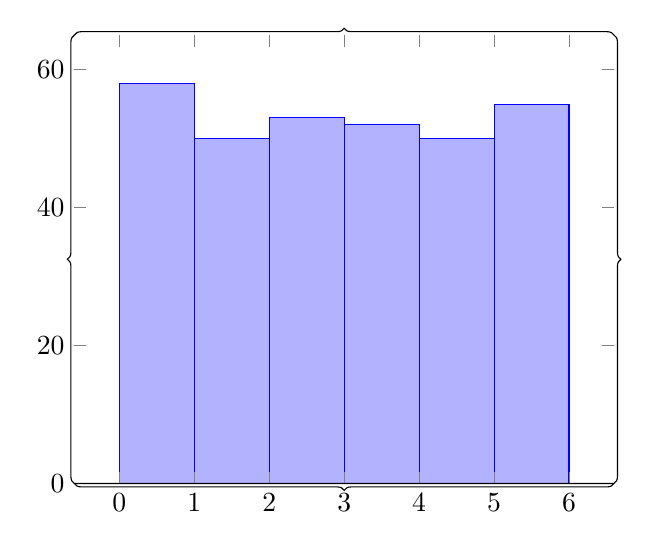
\begin{tikzpicture}
\begin{axis}[
    ymin=0, ymax=65,
    minor y tick num = 0,
    area style,
    ]
\addplot+[ybar interval,mark=no] plot coordinates { (0, 58) (1, 50) (2, 53) (3, 52) (4, 50) (5, 55) (6, 57) };
\end{axis}
\end{tikzpicture}
\end{frame}

\begin{frame}
\frametitle{Understand the Distribution of Continuous Data}
How about real value data, $[-1.407, 0.412, -1.198, 1.552, ...]$? 

\vspace{3mm}
Count the number of data points that falls into the intervals of $[-2, -1.5), [-1.5, -1.0), ... [0, 0.5), [0.5, 1) ...$

%---------------------------------------------------------------%
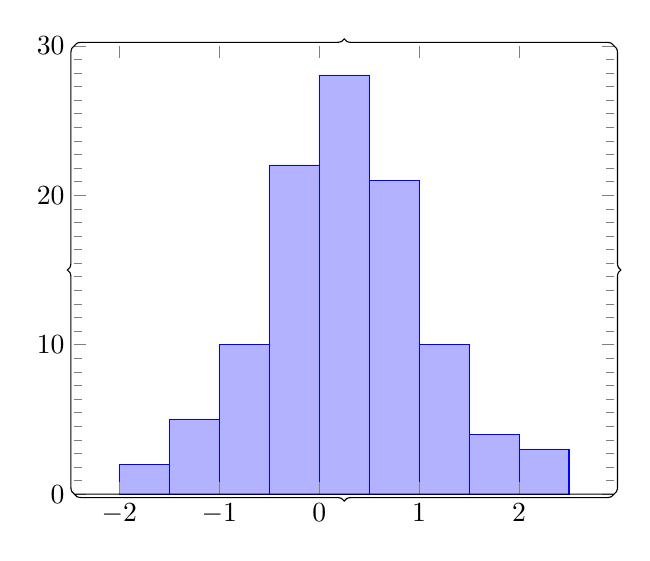
\begin{tikzpicture}
\begin{axis}[
    ymin=0, ymax=30,
    minor y tick num = 10,
    area style,
    ]
\addplot+[ybar interval,mark=no] plot coordinates { (-2, 2) (-1.5, 5) (-1, 10) (-0.5, 22) (0, 28) (0.5, 21) (1,10) (1.5, 4) (2, 3) (2.5, 1)};
\end{axis}
\end{tikzpicture}
\end{frame}


\begin{frame}
\frametitle{Histogram and Empirical Probability Distribution}
\begin{itemize}
\item For data of discrete values, count the number of data occured at each discrete value $N_i$. The total number of data points $N=\sum_{i}N_i$. The empirical probability mass function is given by $$P(x_i)=\frac{N_i}{N}$$
\item For data of continous values, define k equal-sized-bins (e.g. $[x_i-\Delta x, x_i+\Delta x)$, i=1, 2, 3, ...k). Count the number of data belong to each bin $n_i$, the total number of data points $n=\sum_{i}^{k}n_i$. The empirical probability distribution is given by $$P(x_i-\Delta x \leq x < x_i+\Delta x )=\frac{n_i}{n}$$

\end{itemize}
\end{frame}



\begin{frame}
\frametitle{Calculate Mean using Empirical Probability Distribution}

\begin{itemize}
\item Discrete random variable: $$\mu=\sum_{i=1}^k x_i P(x_i)=\frac{\sum_{i=1}^k x_i N_i}{N}$$

This last term of the equation is the same as the arithmic mean of the data points

\end{itemize}
\end{frame}



\begin{frame}
\frametitle{Calculate Mean using Empirical Probability Distribution}

\begin{itemize}


\item Continuous random variable:
\begin{align*}
 \mu &= \sum_{i=1}^k x_i f(x_i-\Delta x \leq x < x_i+\Delta x )(2\Delta x)\\
     &=\sum_{i=1}^k x_i P(x_i-\Delta x \leq x < x_i+\Delta x )\\
     &=\frac{\sum_{i=1}^k x_i n_i}{n}
\end{align*}

This last term of the equation is the approximately arithmic mean of the data points because $x_i n_i \approx \sum_{d \in [x_i-\Delta x, x_i+\Delta x)}d$, $d \in [x_i-\Delta x, x_i+\Delta x)$ denotes the data points belong to the bin $[x_i-\Delta x, x_i+\Delta x)$

\end{itemize}

\end{frame}


\begin{frame}
\frametitle{Histogram and Empirical Probability Distribution}
\begin{center}
 Demo in Python
\end{center}
\end{frame}


\begin{frame}
\frametitle{Statistical Description of Data}

\begin{tabular} { c c c c c c}
 logitude & lattitude & houseAge  &medianHouseValue&oceanProx\\ 
-122.23	&37.88	&41 &452600.0	&NEAR BAY\\
-122.22	&37.86	&21	&358500.0	&NEAR BAY\\
-122.24	&37.85	&52 &352100.0	&NEAR BAY\\
... & ... & ... & & &
\end{tabular}

\vspace{5mm}
Is "medianHouseValue" a random variable? 

\end{frame}

\section{Common Probability Distribution}
\begin{frame}
\begin{center}
\bf{Common Probability Distribution }
\end{center}
\end{frame}


\begin{frame}
\frametitle{Bernoulli Distribution}
Consider a random variable X that can take value 1 with probability p and 0 with probability 1-p.

$$    
P(x) =
    \left\{
        \begin{array}{cc}
                p & \mathrm{if\ } x=1 \\
                1-p & \mathrm{if\ } x=0 \\
        \end{array} 
    \right.
$$
The mean of $X$ is 
$$
E[X]=p
$$

The variance of $X$ is also
$$
E[(X-\mu)^2]=p(1-p)
$$
\end{frame}

\begin{frame}
\frametitle{Binomial Distribution}
Consider a random event that is composed of n independent experiments, whose outcome could either be succuess (1) or failure (0). The probability of success is $p$ and faliure $1-p$. The corresponding random variable X can be described as

$$ P(x) =  {{n}\choose{k}} p^xq^{n-x}, x=0, 1, 2, ...n$$
The mean of $X$ is 
$$
E[X]=np
$$

The variance of $X$ is also
$$
E[(X-\mu)^2]=np(1-p)
$$
\end{frame}

\begin{frame}
\frametitle{Poisson Distribution}
Consider a random event, the number of occurence within a given interval can be x = 0, 1, 2, 3 ... (e.g. No. of car accidents occurs in a day in MO). The distribution of the discrete random variable X can be described as 
$$
P\left( x \right) = \frac{{e^{ - \lambda } \lambda ^x }}{{x!}}, x = 0, 1, 2, ..
$$

The mean of $X$ is 
$$
E[X]=\lambda
$$

The variance of $X$ is also
$$
E[(X-\mu)^2]=\lambda
$$
\end{frame}

\begin{frame}
\frametitle{Poisson Distribution}
Consider a random event, the number of occurence within a given interval can be x = 0, 1, 2, 3 ... (e.g. No. of car accidents occurs in a day in MO). The distribution of the discrete random variable X can be described as 
$$
P\left( x \right) = \frac{{e^{ - \lambda } \lambda ^x }}{{x!}}, x = 0, 1, 2, ..
$$

The mean of $X$ is 
$$
E[X]=\lambda
$$

The variance of $X$ is also
$$
E[(X-\mu)^2]=\lambda
$$
\end{frame}

\begin{frame}
\frametitle{Uniform Distribution}

A uniform distribution is given by
\begin{align*}
f(x) =
    \left\{
        \begin{array}{cc}
              0 & \mathrm{if\ } x<a \\
              \frac{1}{b-a}  & \mathrm{if\ } a\leq x \leq b \\
              0 & \mathrm{if\ } x>b \\
        \end{array} 
    \right.
\end{align*}

\begin{center}
\begin{tikzpicture}
\tkzInit[xmax=0.8,xstep=0.2,ymax=0.65,ystep=0.2]
\tkzDrawX[noticks,label={$x$}]
\tkzDrawY[noticks,label={$f(x)$}]
\tkzDefPoint(0.2,0.6){A}
\tkzDefPoint(0.6,0.6){B}
\tkzDefShiftPoint[A](-90:3){AB}
\tkzDefShiftPoint[B](-90:3){BB}
\tkzDefShiftPoint[AB](0:-0.8){ABL}
\tkzDefShiftPoint[BB](0:0.8){BBR}
\tkzPointShowCoord[xlabel=$a$,ylabel=$\frac{1}{b-a}$](A)
\tkzPointShowCoord[xlabel=$b$](B)
\tkzDrawSegments[color=black,thick](A,B AB,ABL BB,BBR)
\tkzDrawPoints[color=black,fill=black,size=6pt](A,B)
\tkzDrawPoints[color=black,fill=white,size=6pt](AB,BB)
\end{tikzpicture}
\end{center}
\end{frame}

\begin{frame}
\frametitle{Gaussian Distribution}
A continuous random variable $Z$ is called a standard normal if
$$f(Z) = \frac{1}{\sqrt{2\pi}}e^{-z^2/2}$$
The probability of $z\leq z_0$ is given by
$$P(Z\leq z_0) = \int_{-\infty}^{z_{0}}
\frac{1}{\sqrt{2}}e^{-z^2/2}\;dz$$ Let $X=\mu+\sigma Z$. Then $X$
is a normal distribution with parameters $\mu$ and $\sigma^2$. Its
density function is given by
$$f(x) = \frac{1}{\sqrt{2\pi}\sigma}e^{-(x-\mu)^2/2\sigma^2}.$$ 

The mean of $X$: $E[X]=\mu$

The variance of $X$: $E[(X-\mu)^2]=\sigma^2$
\end{frame}


\section{Random Walk, i.i.d, Central Limit Theorem}

\begin{frame}
\begin{center}
\bf{Random Walk, i.i.d, Central Limit Theorem}
\end{center}
\end{frame}



\begin{frame}
\frametitle{Random Walk}
One-dimension random walk: a random process
\begin{itemize}
\item Starting at 0
\item The movement at each step could be either +1 or -1, of equal probability
\end{itemize}
\end{frame}


\begin{frame}
\frametitle{Random Walk}

Define a random variable $B$ that can take value +1 or -1 and have the following random distribution
$$    
P(b) =
    \left\{
        \begin{array}{cc}
                0.5 & \mathrm{if\ } b=1 \\
                0.5 & \mathrm{if\ } b=-1 \\
        \end{array} 
    \right.
$$
The position of a random walk at $t^{th}$ step is a random variable given by 
$$
Z_t=\sum_{i=1}^{t} B_i
$$
\end{frame}

\begin{frame}

\frametitle{Sum of Independent  and  Identically  Distributed (i.i.d)}
Suppose we have n independent random variable $X_1$, $X_2$, $X_3$ ... $X_n$, each have the same probability distribution. We say  $X_1$, $X_2$, $X_3$ ... $X_n$ are
independent  and  identically  distributed (i.i.d). 
The sum of i.i.d random variables given by $Z(n)=\sum_{i=1}^{n} X_i$ has the following properties

\vspace{2mm}

\begin{itemize}
\item $E[Z(n)]=n\mu$;
\item $Var[Z(n)]=n\sigma^2$;
\item When n is large, distribution of Z(n)/n is close to the normal distribution of mean $\mu$ and variance $\sigma^2/n$
\end{itemize}

Here, $\mu$ and $\sigma^2$ are the mean and variance of $X_i$, respectively.


\end{frame}

\begin{frame}
\frametitle{Random Walk}
Since $Z_t$ is the sum of i.i.d, of mean 0 and variance 1, when t is large, $Z_t$ becomes a normal distribution of mean 0 and variance $t$ (why?)

\end{frame}


\end{document}
